\begin{figure}
\begin{subfigure}{.5\textwidth}
  \centering
\begin{class}{IdleShop(id: \integer)}
\begin{state}
m, vmId, self: \integer
\\t: nil | talk
\end{state} 
\\
\begin{init}
\\self = id
\\t = nil
\end{init} 
\\
\begin{op}{switch\_\_\_\_\ then\ ActiveShop}
\Delta (t)
\\x?: nil | talk
\ST
x? = t'
\end{op}
\end{class}
  \caption{1a}
  \label{fig:sfig1}
\end{subfigure}%
\begin{subfigure}{.5\textwidth}
  \centering
\fbox{  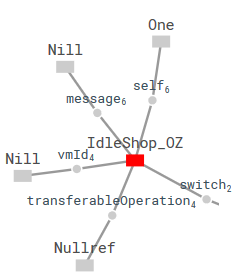
\includegraphics[width=.8\linewidth]{./images/transformational_semantics_of_oz/idleShop_OZ.png}}
  \caption{1b}
  \label{fig:sfig2}
\end{subfigure}
\vspace{2em}

\begin{subfigure}{1\textwidth}
  \centering
\lstinputlisting[backgroundcolor=\color{white},caption={ABC code: IdleShop OZ as a processes.},captionpos=b, label={idleShop_OZ}]{listings/idleShop_OZ.abc}
  \caption{1b}
  \label{fig:sfig3}
\end{subfigure}
\caption{transforming IdleShop}
\label{fig:fig}
\end{figure}